\documentclass[10pt,a4paper]{article}
\usepackage[margin=1.2cm,top=1.1cm,bottom=1.3cm]{geometry}
\usepackage{iftex}
\ifPDFTeX\usepackage[T1]{fontenc}\usepackage[utf8]{inputenc}\usepackage{lmodern}\else\usepackage{fontspec}\fi
\usepackage{microtype,graphicx,booktabs,caption,enumitem,float,hyperref}
\hypersetup{hidelinks}
\captionsetup{font=small,labelfont=bf,skip=2pt}
\setlist{nosep,leftmargin=*}
\setlength{\parskip}{2pt}\setlength{\parindent}{0pt}
\setlength{\textfloatsep}{6pt}\setlength{\floatsep}{4pt}\setlength{\intextsep}{4pt}
\graphicspath{{../artifacts/eda/}}
\renewcommand{\topfraction}{0.9}\renewcommand{\bottomfraction}{0.9}\renewcommand{\textfraction}{0.05}\renewcommand{\floatpagefraction}{0.85}\setcounter{totalnumber}{6}\setcounter{topnumber}{4}\setcounter{bottomnumber}{4}
\newcommand{\sect}[1]{\vspace{3pt}{\large\bfseries #1}\par\vspace{1pt}}

\begin{document}
{\Large\bfseries Early Fake News Detection: datasets and exploratory analysis}\\[2pt]
Michał Pokładowski, Marek Olejniczak, Tomasz Preś, Jędrzej Pluta\\
{\small Semantic Web and Social Networks \textbullet{} Milestone 2 \textbullet{} 09.11.2026 \hfill Repository: \url{https://github.com/michaelo-ponteski/SWSN}}

\sect{1. Chosen datasets}
We classify a news item or claim as fake or real from only the \emph{first part} of its spread on Twitter
(first $h$ hours or first $k$ engagements), which requires propagation trees with a timestamp on every node.
We use four datasets from two independent sources (Table~\ref{tab:data}).
\textbf{PolitiFact} and \textbf{GossipCop} come from UPFD~[1], the dataset of our main paper
(politics and celebrity news; per-node timestamps from the UPFD authors' repository).
\textbf{Twitter15/16}~[2] differ from the main paper: a different collection and domain (rumour claims), four veracity
classes, larger and much faster cascades, and no user features. They let us test whether conclusions transfer beyond UPFD.
For binary experiments we map \emph{false}$\to$fake, \emph{true}+\emph{non-rumor}$\to$real and drop \emph{unverified}
(veracity unknown), which makes Twitter ${\sim}$2:1 real:fake.

\begin{table}[h]\centering\footnotesize
\caption{Datasets after preprocessing. Labels: real/fake (UPFD), non-rumor/false/true/unverified (Twitter). Span = median time from first to last engagement.}\label{tab:data}
\begin{tabular}{llrlrrll}\toprule
Dataset & Source & Cascades & Labels & Mean nodes & Span & Node & Node features\\\midrule
PolitiFact & UPFD [1] & 314 & 157 / 157 & 131 & 219 d & post & user history (BERT, spaCy), profile\\
GossipCop & UPFD [1] & 5464 & 2732 / 2732 & 58 & 9 d & post & as above\\
Twitter15 & Ma et al. [2] & 1490 & 374 / 370 / 372 / 374 & 402 & 8 d & user & none (source text only)\\
Twitter16 & Ma et al. [2] & 818 & 205 / 205 / 207 / 201 & 425 & 8 d & user & none (source text only)\\\bottomrule
\end{tabular}
\end{table}

\sect{2. Data model and preprocessing}
All datasets are converted (\texttt{src/build\_data.py}; analysis in \texttt{notebooks/eda.ipynb}) into one format: a rooted tree per cascade (root = news or source tweet, edge = parent
$\to$ child propagation) with nodes sorted by time, so that parent time $\le$ child time. Hence every early window is a
prefix of the node list and always a connected tree, and the same window can be given to a model either as a
\emph{graph} or as a time-ordered \emph{sequence} (Fig.~\ref{fig:model}), which is exactly the comparison our project makes.
Raw Twitter trees are not strict trees: ${\sim}$1\% of nodes have several candidate parents, which causes 98\% of
time-inverted edges. We keep the most recent earlier parent, drop self-loops, and clamp 736 posts that predate the source
tweet to $t{=}0$. Every fix is a column or flag (raw data untouched). We also flag leakage sources: 169 cascades
occur in both Twitter15 and Twitter16, some source texts repeat, and UPFD contains 39 groups of different news items
with identical cascades.

\begin{figure}[!htb]\centering
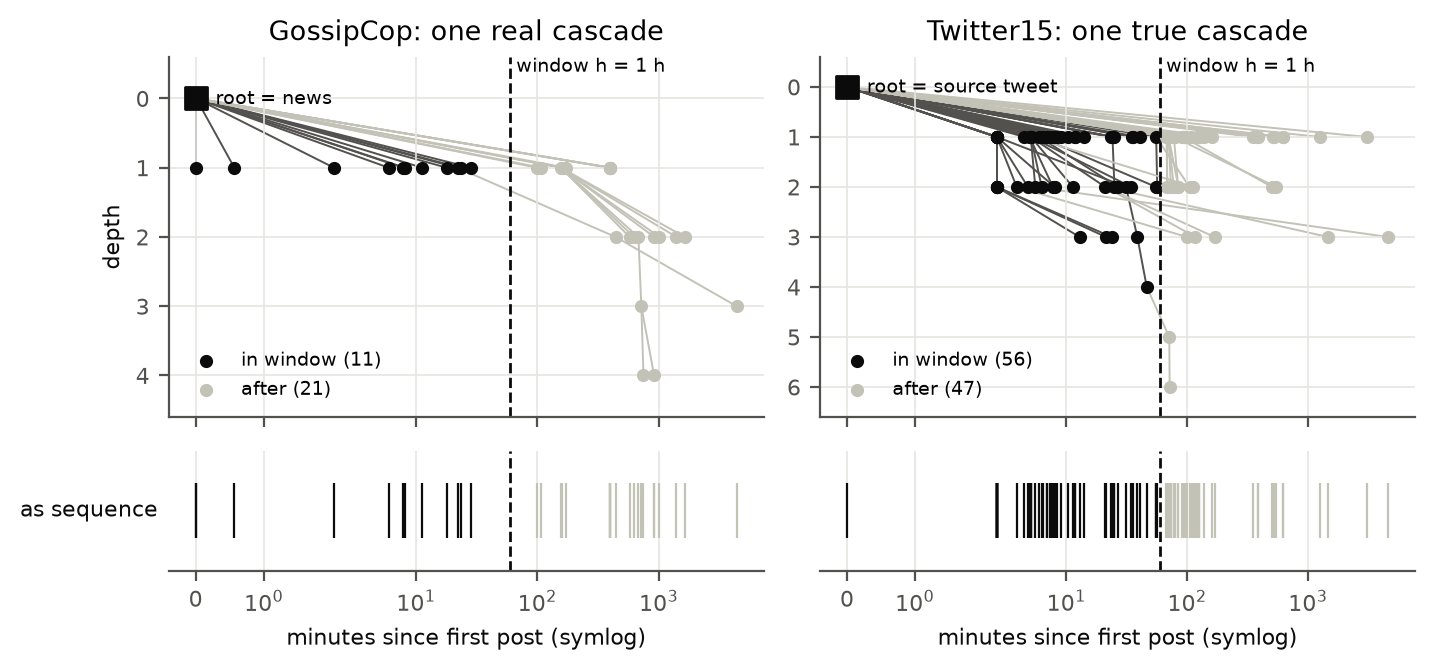
\includegraphics[width=11.5cm]{fig0_cascade_example.png}
\caption{Two real cascades as trees (x: time, y: depth) and as sequences. Left of the dashed line: the input of a 1-hour early detector.}\label{fig:model}
\end{figure}

\sect{3. Basic analysis: size and shape}
Cascade size depends on the class, but not in the same direction everywhere (Fig.~\ref{fig:size}): fake cascades are
smaller in GossipCop (median 22 vs 70 nodes) and Twitter (${\sim}$210 vs ${\sim}$350), but larger in PolitiFact (104 vs 58).
Trees are shallow and star-like: the median share of nodes attached directly to the root is 0.6--0.9 and 70\% of GossipCop
cascades have depth 2; the depth distributions of the two classes overlap strongly.

\begin{figure}[!htb]\centering
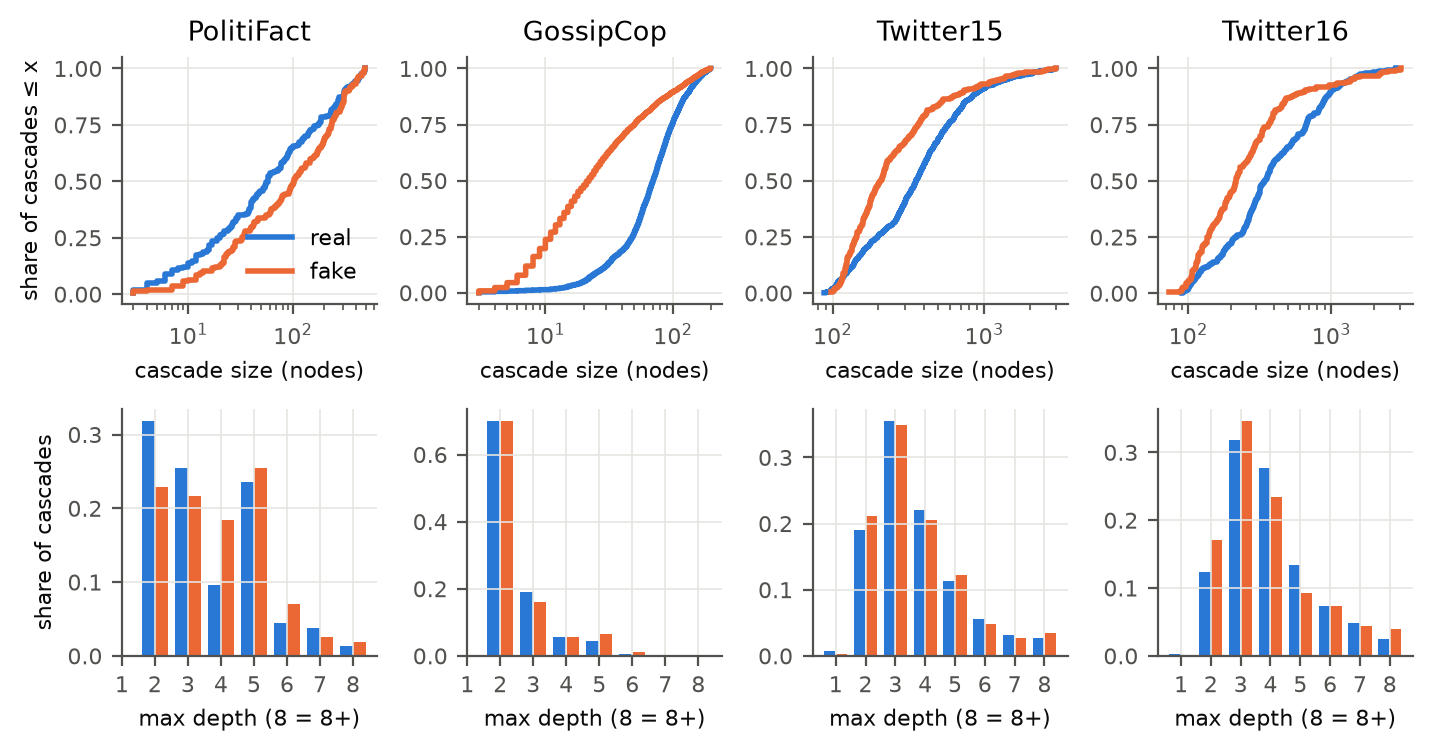
\includegraphics[width=12cm]{fig1_size_depth.png}
\caption{Top: cumulative distribution of cascade size; bottom: distribution of maximum depth (binary labels).}\label{fig:size}
\end{figure}

\sect{4. Specific analysis: what can be seen early?}
\textbf{Growth speed differs by orders of magnitude} (Fig.~\ref{fig:growth}). After 1\,h a Twitter cascade has ${\sim}$60\%
of its final size (median ${\sim}$160 engagements), GossipCop 25\% and PolitiFact 5\% (median 2 engagements); real
PolitiFact cascades keep growing for years. A fixed ``first $h$ hours'' is therefore not comparable across datasets, so we
will use per-dataset time grids together with first-$k$ windows.

\begin{figure}[!htb]\centering
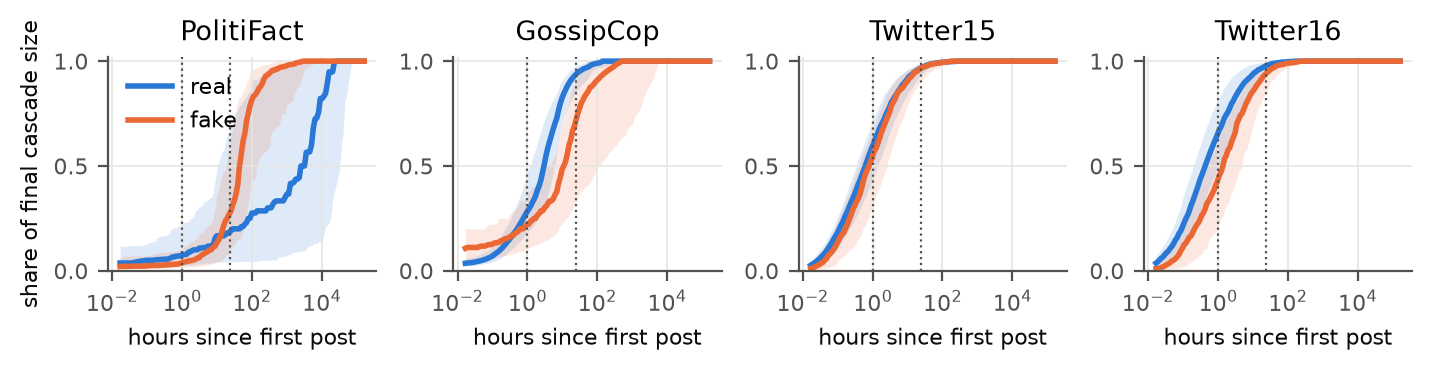
\includegraphics[width=13.5cm]{fig2_growth.png}
\caption{Share of the final cascade size observed $t$ hours after the first post (median and interquartile range per class).}\label{fig:growth}
\end{figure}

\textbf{Simple activity features are strong early, structure is not} (Fig.~\ref{fig:auc}). The number of engagements in
the window alone reaches ROC AUC 0.89 on GossipCop after 6\,h (0.79 on full cascades) and 0.81 on Twitter16 after only
10 minutes (0.66 on full cascades): early activity is \emph{more} informative than the whole cascade. Tree shape (maximum
depth, share of root children) stays at AUC 0.5--0.6 in most windows, because early trees are mostly stars.
PolitiFact separates only after several days.

\begin{figure}[!htb]\centering
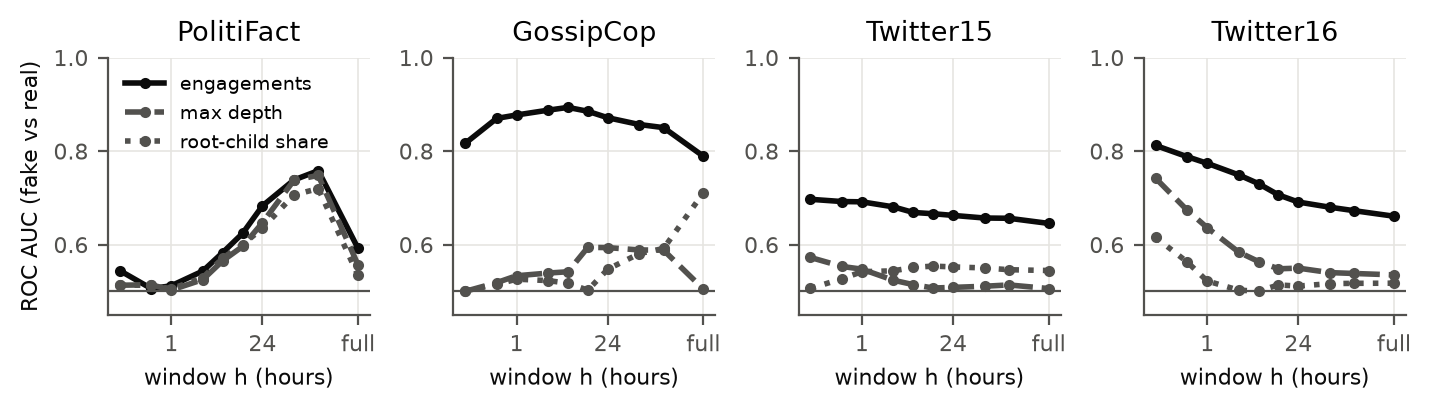
\includegraphics[width=13.5cm]{fig3_auc_by_window.png}
\caption{Separability (ROC AUC, direction-free) of single features computed on the first $h$ hours; ``full'' = whole cascade.}\label{fig:auc}
\end{figure}

\textbf{Fake content starts slower here} (Fig.~\ref{fig:speed}). The 5th engagement arrives after a median of 8\,min for
real and ${\sim}$5\,h for fake GossipCop news (AUC 0.85 from this one number), and after 0.6--0.7 vs 1.5--1.7\,min on
Twitter. This contradicts the common ``fake spreads faster'' finding~[3] at the start of a cascade; a likely reason is that
real stories come from large mainstream accounts. PolitiFact behaves differently (fake becomes faster after some hours).

\begin{figure}[!htb]\centering
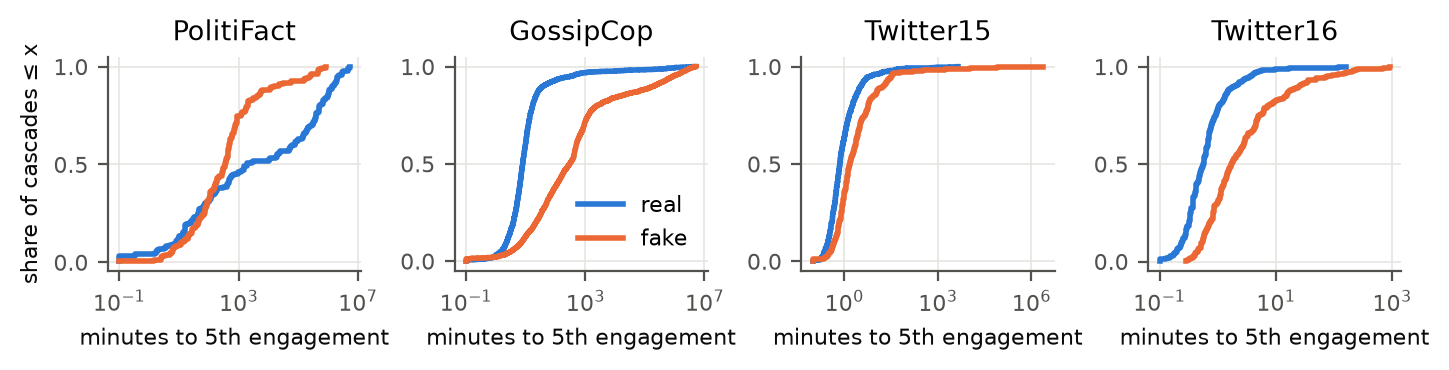
\includegraphics[width=13.5cm]{fig4_time_to_k.png}
\caption{Cumulative distribution of the time until the 5th engagement.}\label{fig:speed}
\end{figure}

\textbf{Users and splits.} 10--21\% of users take part in several cascades, and 60--82\% of them only ever appear in one
class, against 30--47\% after shuffling the labels. User identity is thus a strong signal (it explains why UPFD's
user-history features work), but also a leakage channel. The official PyG split of UPFD is small
(62 training cascades in PolitiFact) and puts 18 of the 39 duplicate-cascade groups on both sides of the split.


{\footnotesize\textbf{References.}
[1] Y.~Dou et al., User Preference-aware Fake News Detection, SIGIR 2021.
[2] J.~Ma, W.~Gao, K.-F.~Wong, Detect Rumors in Microblog Posts Using Propagation Structure via Kernel Learning, ACL 2017.
[3] S.~Vosoughi, D.~Roy, S.~Aral, The spread of true and false news online, Science 359, 2018.\par}
\end{document}
